\section{Summary}

\begin{frame}{Summary}
\uncover<1->{
    \begin{figure}
        \centering
        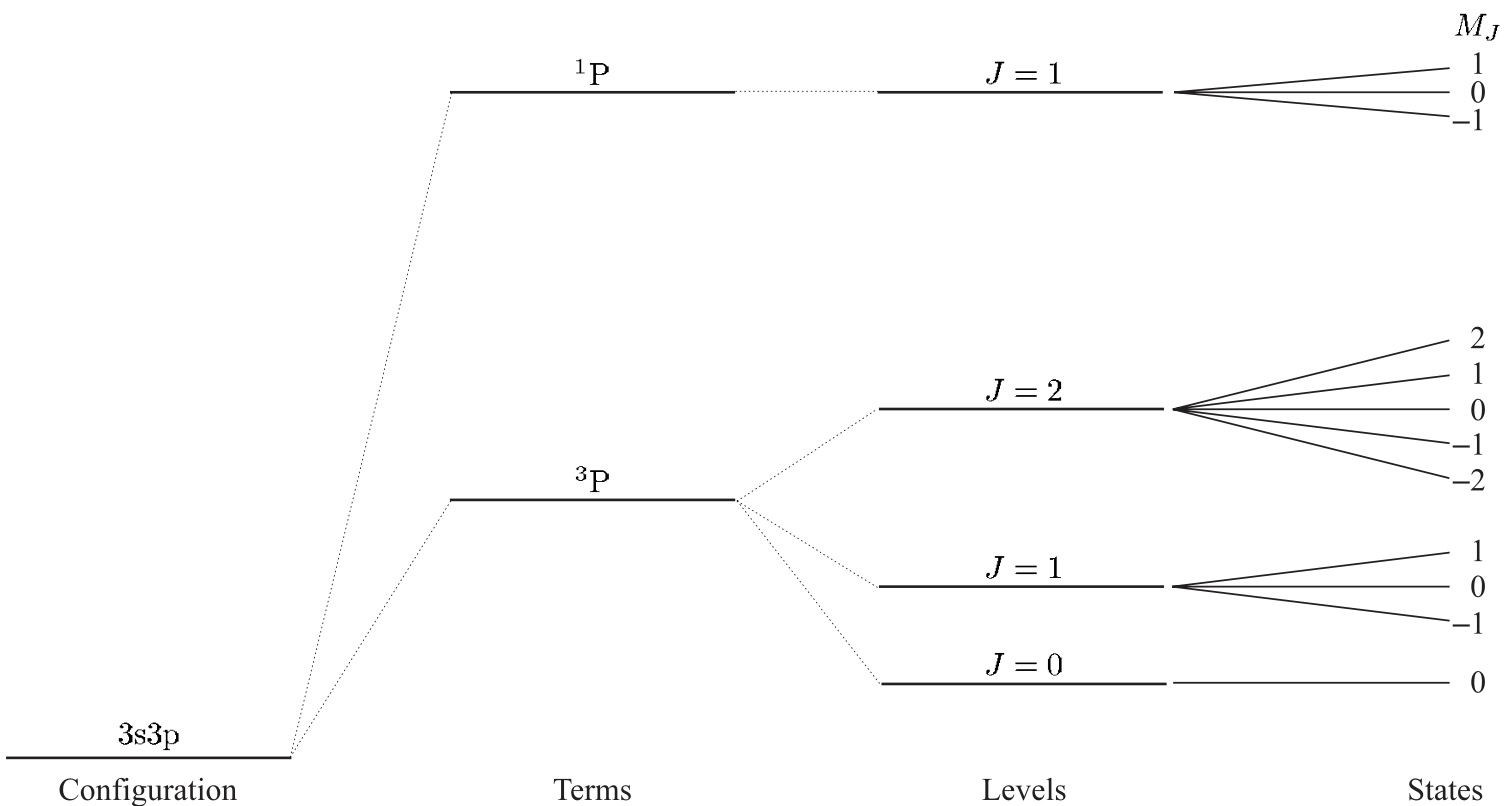
\includegraphics[scale=0.25]{fig/fig 5.16.png}
        \caption{The hierarchy of atomic structure for the 3s3p configuration of an alkaline earth metal atom.}
    \end{figure}}
\uncover<2->{
    Break down:\\
    (a) The residual electrostatic interaction is not small compared to the energy gap between the configurations.\\
    (b) The jj-coupling scheme is a better approximation than LS-coupling. \\
    (c) The Paschen–Back effect arises.}
\end{frame}